\documentclass{article}\usepackage[]{graphicx}\usepackage[]{color}
%% maxwidth is the original width if it is less than linewidth
%% otherwise use linewidth (to make sure the graphics do not exceed the margin)
\makeatletter
\def\maxwidth{ %
  \ifdim\Gin@nat@width>\linewidth
    \linewidth
  \else
    \Gin@nat@width
  \fi
}
\makeatother

\definecolor{fgcolor}{rgb}{0.345, 0.345, 0.345}
\newcommand{\hlnum}[1]{\textcolor[rgb]{0.686,0.059,0.569}{#1}}%
\newcommand{\hlstr}[1]{\textcolor[rgb]{0.192,0.494,0.8}{#1}}%
\newcommand{\hlcom}[1]{\textcolor[rgb]{0.678,0.584,0.686}{\textit{#1}}}%
\newcommand{\hlopt}[1]{\textcolor[rgb]{0,0,0}{#1}}%
\newcommand{\hlstd}[1]{\textcolor[rgb]{0.345,0.345,0.345}{#1}}%
\newcommand{\hlkwa}[1]{\textcolor[rgb]{0.161,0.373,0.58}{\textbf{#1}}}%
\newcommand{\hlkwb}[1]{\textcolor[rgb]{0.69,0.353,0.396}{#1}}%
\newcommand{\hlkwc}[1]{\textcolor[rgb]{0.333,0.667,0.333}{#1}}%
\newcommand{\hlkwd}[1]{\textcolor[rgb]{0.737,0.353,0.396}{\textbf{#1}}}%

\usepackage{framed}
\makeatletter
\newenvironment{kframe}{%
 \def\at@end@of@kframe{}%
 \ifinner\ifhmode%
  \def\at@end@of@kframe{\end{minipage}}%
  \begin{minipage}{\columnwidth}%
 \fi\fi%
 \def\FrameCommand##1{\hskip\@totalleftmargin \hskip-\fboxsep
 \colorbox{shadecolor}{##1}\hskip-\fboxsep
     % There is no \\@totalrightmargin, so:
     \hskip-\linewidth \hskip-\@totalleftmargin \hskip\columnwidth}%
 \MakeFramed {\advance\hsize-\width
   \@totalleftmargin\z@ \linewidth\hsize
   \@setminipage}}%
 {\par\unskip\endMakeFramed%
 \at@end@of@kframe}
\makeatother

\definecolor{shadecolor}{rgb}{.97, .97, .97}
\definecolor{messagecolor}{rgb}{0, 0, 0}
\definecolor{warningcolor}{rgb}{1, 0, 1}
\definecolor{errorcolor}{rgb}{1, 0, 0}
\newenvironment{knitrout}{}{} % an empty environment to be redefined in TeX

\usepackage{alltt}
%\usepackage[margin=1in]{geometry}   % set up margins
\usepackage[vmargin=1in,hmargin=1in]{geometry}
\usepackage{tikz}
\usepackage{booktabs}

\usepackage[backend=bibtex]{biblatex}
\IfFileExists{upquote.sty}{\usepackage{upquote}}{}


\thispagestyle{empty}
\begin{center}
\begin{minipage}{1.2\linewidth}
    \centering
 %   \rule{0.4\linewidth}{0.15\linewidth}\par
    \vspace{3cm}
%Thesis title
    \textbf{{\uppercase{\Large German Credit Data Scoring using R\par}}}
    \vspace{2cm}
    %Degree
    {\Large Business Data Analytics Project Report\par}
    \vspace{2cm}
    %University logo
   \hspace{1.5cm} 
\includegraphics[width=0.35\linewidth]{hyderabad-university-publishes-mtech.jpg}\newline
    
%Author's name
  \centering
    {\Large Laltendu Das [15MCMI22]\par}
    {\Large Uma Revathi [15MCMI22]\par}
    {\Large  Rosni K V [15MCMI15]\par}
    \vspace{1cm}
    
    %Author's name
    {\textit{\hspace{1cm}Under the Guidance of} \par}
    {\Large Dr. V.Ravi, Associate Professor, IDRBT \par}
    \vspace{2cm}
    \centering
%Date
    {\textbf{\Large November 2015}}
\end{minipage}
\end{center}
\clearpage

\newpage
\renewcommand{\contentsname}{\centering Table of Contents}
\newline
\tableofcontents
\newpage
%\renewcommand{\listfigurename}{\centering List of Figures}
\listoffigures
\newpage
%\renewcommand{\listoftables}{\centering List of Tables}
\listoftables

\begin{document}
%preamble



\title {An Attractive Template of a Reproducible Data Analysis Document for an Awesome Class Project}
\author{Mahbubul Majumder, PhD\\ Department of Mathematics\\ University of Nebraska at Omaha }

\maketitle



\begin{abstract}This first sentence of the abstract starts with a little background of the problem. The second sentence starts describing the problem with some motivation. If needed we add another sentence to increase the reader's interest and clarity. After the problem description is over, we need to describe what we have done, how we did it and what results we obtained. We include any challenges we face and solution of that challenges we made. We describe any experiment we did with their findings. We also clearly mention how our results or methods are better than any existing results or methods. Sometimes we like to mention how this work opens up some future works. Abstract should not be more than a paragraph preferably having less than 200 words.
\end{abstract}

%\tableofcontents

\section{Introduction} The first sentence of this section is so attractive that it made the reader concentrate on reading. The second sentence is so great that it made the reader forget the date. Rest of the sentences are so nice that at the end of the paragraph the reader can't just wait to see what is coming on the next paragraph. At this point reader does not mind if it gets a little technical.  \\

The first sentence of any paragraph presents a clear message. The rest of the sentences just describe that idea and establish the facts so that the reader see the logical conclusion of the paragraph. The last sentence of the paragraph connects the following paragraphs or section.  \\

Add some motivational pictures in this section whenever possible. This will provide the reader some relief from reading text after text. For example Figure \ref{fig:nice-plot} indeed make us happy that we have something else to concentrate. This motivational picture does not need to be generated from the data you are going to analyze. Notice that we added the \textbf{R} codes of generating the Figure~\ref{fig:nice-plot}.

%If we don't want to display the R codes, we just put option \texttt{echo=FALSE} in the head of the chunk. To add caption for the figure we write the caption in \texttt{fig.cap=`my figure captions'}.

\begin{knitrout}
\definecolor{shadecolor}{rgb}{0.969, 0.969, 0.969}\color{fgcolor}\begin{kframe}
\begin{alltt}
\hlkwd{plot}\hlstd{(women)}
\end{alltt}
\end{kframe}\begin{figure}[hbtp]

{\centering 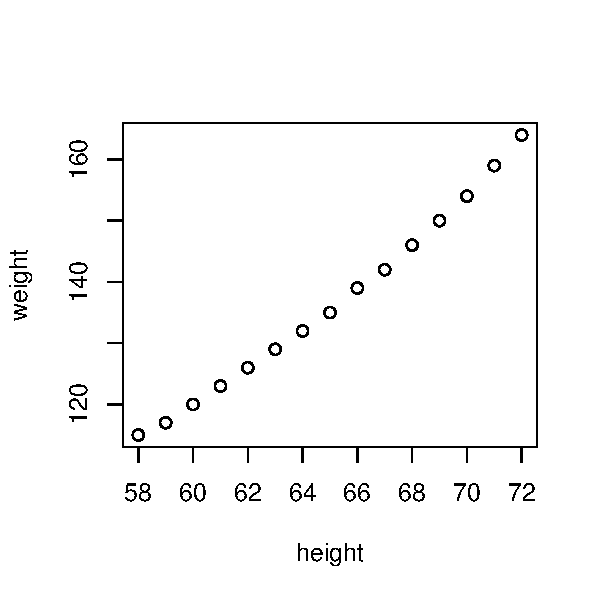
\includegraphics[width=.45\linewidth]{figure/nice-plot-1} 

}

\caption[My awesome figure caption really describes what this figure is about and what we see in this figure]{My awesome figure caption really describes what this figure is about and what we see in this figure. Also notice that the figure size is kept in such a way that it fits in the text nicely - not too big nor too small}\label{fig:nice-plot}
\end{figure}


\end{knitrout}

Also please don't forget to explain in details about what this figure is telling. It is really a bad idea not to say anything about the figure when you added it. Its like a product you are selling to someone who don't want to buy it. So, you have to be very serious about selling it with convincing argument.

\subsection{Preparing this document} This whole document is prepared using \textbf{R}  \cite{R-base} package \texttt{knitr} \cite{R-knitr}. It is a dynamic document and reproducible any number of times for any data sets. To start our work conveniently we need to install \textbf{R}, \texttt{RStudio} and \LaTeX{} \cite{lamport94} . Once our installation is done we will configure \texttt{RStudio} to work with \texttt{knitr}. For this first install \texttt{knitr} using command \texttt{install.packages("knitr")} and include the \texttt{knitr} library by command \texttt{library(knitr)}. Once \texttt{knitr} is installed go to the \texttt{RStudio} menu \texttt{Tools > Global Options...Sweave} and change `Weave Rnw files using' to indicate \texttt{Knitr}.\\

Now we are ready to create our first document using \texttt{knitr}. Go to \texttt{File > New File > R Sweave} and it will start with a new template for a document. If you save this minimal template it will be saved as a \texttt{.Rnw} file. Now we can just start filling the template with our texts. To create a human readable pdf file from \texttt{.Rnw} we just click on \texttt{Compile PDF} in \texttt{RStudio} toolbar. \\

{\bf PDF latex failure:} If you encounter any problem such as \texttt{Running pdflatex on ...failed} it could be due to the bibliography. To solve that problem what you can do is: Go back to the folder where you saved your \texttt{.Rnw} file and find the \texttt{.tex} file that is created automatically. Now run the \texttt{.tex} file from \LaTeX{} editor to create the pdf. Once you do this multiple times your bibliographies would be updated and you will be ready to work from \texttt{RStudio} as long as you don't change any object that has references in the file. There may be a better solution for this, but so far this worked for me. \\

The solution for this problem: just add \texttt{\textbackslash usepackage[backend=bibtex]{biblatex}} in your preamble of the \texttt{.Rnw} file.

\section{About the data} In this section we would like to describe the data we are going to use for the analysis. For example we intend to study the trees data that comes with default \textbf{R} installation. There are 31 data points and 3 variables in this data set. The variables are Girth, Height, Volume. The data may not be tidy and we may have to prepare the data before our analysis can be done. We will discuss how we prepared the data in the following section.

\subsection{Preparing data} You invested lot of times preparing your data for exploration. Why not you describe what you did and how you did. You may add your R codes so that others know what exactly you did. For example let us view the summary of the data as below.

\begin{knitrout}
\definecolor{shadecolor}{rgb}{0.969, 0.969, 0.969}\color{fgcolor}\begin{kframe}
\begin{alltt}
\hlkwd{summary}\hlstd{(trees)}
\end{alltt}
\begin{verbatim}
##      Girth           Height       Volume     
##  Min.   : 8.30   Min.   :63   Min.   :10.20  
##  1st Qu.:11.05   1st Qu.:72   1st Qu.:19.40  
##  Median :12.90   Median :76   Median :24.20  
##  Mean   :13.25   Mean   :76   Mean   :30.17  
##  3rd Qu.:15.25   3rd Qu.:80   3rd Qu.:37.30  
##  Max.   :20.60   Max.   :87   Max.   :77.00
\end{verbatim}
\end{kframe}
\end{knitrout}

Try to avoid putting raw output like this in your final report. Instead make a clean table as shown in table \ref{summary-data}. If you have to keep some raw output of your analysis please put them in a section called appendix at the end of the document. If you really believe that you have to put them here, you can do that and thats why we have this example here.

\subsection{What is funny} This section may not be necessary. But if you notice something  about the data that does not make any sense you can mention them in a section like that. Or if you think of anything interesting about the data, just discuss them here.

\section{Methods} This section will include the methods you are planning to use for your analysis. You should include some theoretical justification here. For example, why you think the method is applicable, what are the assumptions about the methods, whether your data satisfies those assumption or not etc. 

\subsection{The model}
These theories may require you to type mathematical equations and we need to refer them in the text like equation \ref{eq:reg}.

\begin{equation} \label{eq:reg}
 Y = \beta_0 + \beta_1 X + \epsilon
\end{equation}
where $\epsilon \sim N(0,1)$.

You should discuss the exploratory steps and the logical conclusion of adopting equation \ref{eq:reg} for fitting to your data. Clearly mention the conditions and the assumptions of the model. Do not write any result of the model in this section. This section is only for theoretical discussion and any results of these models should be discussed in results section.

\subsection{Data product} You may end up building a data product in your project. You may discuss about the plan here.

\section{Results} In result section you can start with an overview of what you have found during the exploration of data. 

\subsection{Including tables}
Include some summary tables of the data as as shown in table \ref{summary-data}. Make sure you discuss about the table you have included and explain the facts it is revealing. You have to sell your table in a way that the reader will understand that this table was awesome and it reveals a fact the reader would otherwise not recognize.\\

Notice that we used the function \texttt{xtable()} form the \textbf{R} package \texttt{xtable} \cite{xtab} to generate a pretty table. \texttt{knitr} does this using \LaTeX{} codes generated by \texttt{xtable} and automatically put it in a nicer we and we don't have to worry about its position. Also notice how we write the caption of the table as well as refer the table \ref{summary-data} from the text.

\begin{kframe}
\begin{alltt}
\hlcom{# Creating and printing summary data table}
\hlkwd{library}\hlstd{(xtable)}
\hlstd{summary_data} \hlkwb{<-} \hlkwd{apply}\hlstd{(trees,} \hlnum{2}\hlstd{,} \hlkwa{function}\hlstd{(}\hlkwc{x}\hlstd{) \{}
    \hlkwd{return}\hlstd{(}\hlkwd{c}\hlstd{(}\hlkwc{Average} \hlstd{=} \hlkwd{mean}\hlstd{(x),} \hlkwc{Median} \hlstd{=} \hlkwd{median}\hlstd{(x),} \hlkwc{SD} \hlstd{=} \hlkwd{sd}\hlstd{(x),} \hlkwc{Range} \hlstd{=} \hlkwd{range}\hlstd{(x)))}
\hlstd{\})}
\hlkwd{print}\hlstd{(}\hlkwd{xtable}\hlstd{(summary_data,} \hlkwc{digits} \hlstd{=} \hlnum{2}\hlstd{,} \hlkwc{caption} \hlstd{=} \hlkwd{paste}\hlstd{(}\hlstr{"This table caption really"}\hlstd{,}
    \hlstr{"describes what this table is about and what interesting facts it is revealing."}\hlstd{),}
    \hlkwc{label} \hlstd{=} \hlstr{"summary-data"}\hlstd{),} \hlkwc{caption.placement} \hlstd{=} \hlkwd{getOption}\hlstd{(}\hlstr{"xtable.caption.placement"}\hlstd{,}
    \hlstr{"top"}\hlstd{))}
\end{alltt}
\end{kframe}% latex table generated in R 3.2.1 by xtable 1.7-4 package
% Mon Sep 28 22:49:21 2015
\begin{table}[ht]
\centering
\caption{This table caption really describes what this table is about and what interesting facts it is revealing.} 
\label{summary-data}
\begin{tabular}{rrrr}
  \hline
 & Girth & Height & Volume \\ 
  \hline
Average & 13.25 & 76.00 & 30.17 \\ 
  Median & 12.90 & 76.00 & 24.20 \\ 
  SD & 3.14 & 6.37 & 16.44 \\ 
  Range1 & 8.30 & 63.00 & 10.20 \\ 
  Range2 & 20.60 & 87.00 & 77.00 \\ 
   \hline
\end{tabular}
\end{table}


\subsubsection{Book quality table} We can add tables that look like the tables in the book. For this we need to add package \texttt{booktabs} in the preamble of this .Rnw file. This will include a package called \texttt{booktabs} onto \LaTeX. Once we add that we can now put option \texttt{booktabs = TRUE} in the \textbf{R} code as below.

\begin{kframe}
\begin{alltt}
\hlkwd{library}\hlstd{(knitr)}
\hlstd{x} \hlkwb{<-} \hlkwd{head}\hlstd{(mtcars)}
\hlkwd{kable}\hlstd{(x,}\hlkwc{format} \hlstd{=} \hlstr{'latex'}\hlstd{,} \hlkwc{booktabs} \hlstd{=} \hlnum{TRUE}\hlstd{)}
\end{alltt}
\end{kframe}
\begin{tabular}{lrrrrrrrrrrr}
\toprule
  & mpg & cyl & disp & hp & drat & wt & qsec & vs & am & gear & carb\\
\midrule
Mazda RX4 & 21.0 & 6 & 160 & 110 & 3.90 & 2.620 & 16.46 & 0 & 1 & 4 & 4\\
Mazda RX4 Wag & 21.0 & 6 & 160 & 110 & 3.90 & 2.875 & 17.02 & 0 & 1 & 4 & 4\\
Datsun 710 & 22.8 & 4 & 108 & 93 & 3.85 & 2.320 & 18.61 & 1 & 1 & 4 & 1\\
Hornet 4 Drive & 21.4 & 6 & 258 & 110 & 3.08 & 3.215 & 19.44 & 1 & 0 & 3 & 1\\
Hornet Sportabout & 18.7 & 8 & 360 & 175 & 3.15 & 3.440 & 17.02 & 0 & 0 & 3 & 2\\
Valiant & 18.1 & 6 & 225 & 105 & 2.76 & 3.460 & 20.22 & 1 & 0 & 3 & 1\\
\bottomrule
\end{tabular}



\subsection{Including figures} Please don't forget to add nice data plots in your documents. Plots are nice to conveying message and much better than tables. Discuss what facts the figure is revealing and refer the figure from the text as figure \ref{fig:data-plot}.

\begin{knitrout}
\definecolor{shadecolor}{rgb}{0.969, 0.969, 0.969}\color{fgcolor}\begin{kframe}
\begin{alltt}
\hlkwd{plot}\hlstd{(trees)}
\end{alltt}
\end{kframe}\begin{figure}[hbtp]

{\centering 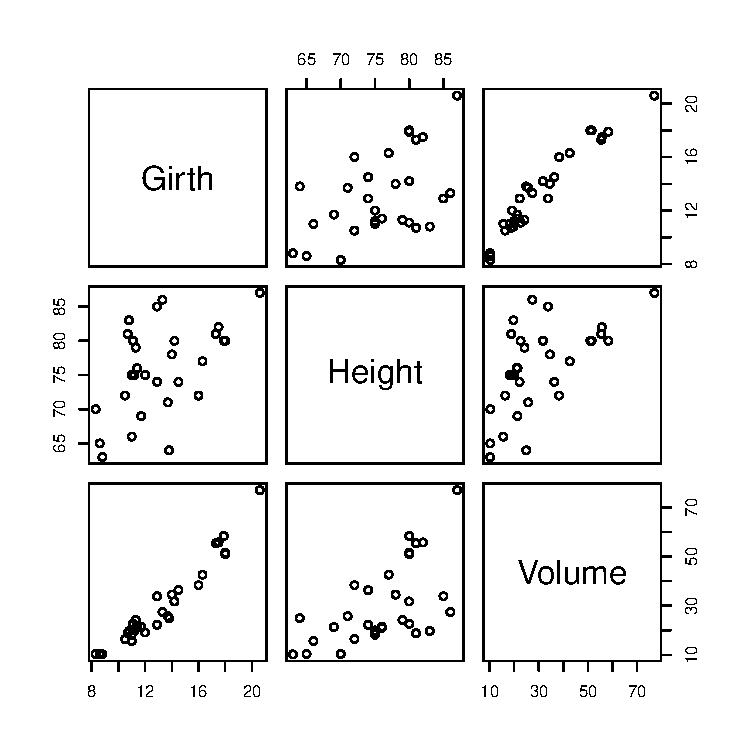
\includegraphics[width=.6\linewidth]{figure/data-plot-1} 

}

\caption[Awesome figure caption]{Awesome figure caption}\label{fig:data-plot}
\end{figure}


\end{knitrout}

\subsection{How the data product works} If you build a data product you may discuss here how it works and what it provides. For data product being your main purpose, your main section may be different from just saying \texttt{Results}. You may think how you rename your sections to naturally fit in your work and the purpose.

\section{Conclusion} The conclusion is an elaboration of your abstract. Here you will discuss what you have done and how. The gist of the results need to be mentioned here. It needs to be convincing and the reader will never regret forgetting the date. Please keep it in mind that there may be readers who only read your conclusion. So, make your conclusion complete so that no reader misses anything even if they don't want to read the whole document.\\

Each paragraph of the conclusion may discuss one result you have found or one concept you are proposing. Discuss your findings and why it is better and how it is compared to any existing methods may exist. \\

Please don't forget to cite the works of others if you used it in your analysis. The citation is important for two reasons. Fist of all it acknowledges the good works other people have done which encourages them keep continue doing their good work. Second, it protects you from plagiarism which is a very nasty task everyone should avoid.\\

There should be one paragraph about the future direction of the work you have done. You would like to make it so fascinating that the reader would wish to be involved in this work in future. \\

Finally this is just a template. Your exact document may have a very different outlook. It demonstrates how you can start to write a document. Our biggest problem is to figure out where to start from. And this documents provides a guide for that. I hope it turns out to be helpful for some of the readers. If you have any comments or concern about this document please let me know so that I can improve this document. 

\begin{thebibliography}{9}

\bibitem{xtab}
    David B. Dahl,
    \emph{xtable: Export tables to LaTeX or HTML},
    R package version 1.7-3,
    http://CRAN.R-project.org/package=xtable, 
    2014

\bibitem{lamport94}
  Leslie Lamport, \emph{\LaTeX: A Document Preparation System}.
  Addison Wesley, Massachusetts,
  2nd Edition, 1994.

\bibitem{R-base}
  R Core Team, \emph{R: A Language and Environment for Statistical Computing},
  R Foundation for Statistical Computing,
  Vienna, Austria, http://www.R-project.org/ ,
  2014
  
\bibitem{R-knitr}
  Yihui Xie
  \emph{knitr: A general-purpose package for dynamic report generation in R},
  http://yihui.name/knitr/, 2014  

\end{thebibliography}

\end{document}
